\chapter{Desenvolvimento} \label{cap:desenvolvimento}

Devido à importância do tema e ao raciocínio apresentado, um método para análise de \index{Vulnerabilidade}vulnerabilidades em redes industriais \index{OPC UA}OPC UA foi desenvolvido. O presente capítulo oferece os principais aspectos da bancada experimental utilizada e o conjunto de estratégias adotados para a realização e desenvolvimento do mesmo, assim como o cronograma proposto para o cumprimento das metas estabelecidas.

\section{Aspectos da Bancada Experimental para Ensaios de Intrusão em Redes OPC UA}

    Nesta seção, toda a estrutura responsável pela aquisição de dados experimentais gerados para auxiliar no desenvolvimento do presente trabalho é descrita. A \autoref{fig:esqBanc} ilustra a composição da estrutura da bancada experimental utilizada, cujos principais componentes são detalhados a seguir:

    \begin{figure}[htbp]
        \caption{\label{fig:esqBanc}Esquema geral da bancada experimental para ensaios de segurança cibernética}
        \begin{center}
            \includegraphics[width=0.6\textwidth]{USPSC-img/bancada-low.png}
        \end{center}
        \legend{Fonte: elaborada pelo autor.}
    \end{figure}

    \subsection{\textit{Hardware}}

    Para simular os ataques cibernéticos, são necessários um conjunto de componentes de \textit{hardware} combinados com ferramentas de \textit{software} específicas. A lista a seguir detalha cada equipamento utilizado.

    \begin{itemize}
        \item \underline{DF63 NG}: representa a nova geração dos controladores multifuncionais da plataforma DFI302 da Nova Smar S/A funcionando como um `\textit{linking device}' para conectar redes H1 independentes e redes Ethernet HSE, especialmente projetado para soluções de controle distribuído em redes industriais. Além de suportar comunicação Modbus, oferece recursos avançados, incluindo redundância `\textit{Hot standby}', comunicação OPC UA nativa, estampa de tempo e configuração por meio da linguagem Ladder conforme IEC 61131. A DF63 NG é altamente versátil, permitindo a instanciação de centenas de blocos funcionais, incluindo blocos flexíveis, e possui um servidor Web integrado para diagnóstico e parametrização;
        \item \underline{Raspberry Pi 4 Modelo B}: são utilizados dois mini-computadores de placa única multiplataforma, configuradas com o sistema operacional Kali Linux, hospedando um cliente e um servidor OPC UA cada. A Raspberry Pi 4 Modelo B representa uma evolução significativa em relação às gerações anteriores, incorporando um processador ARM Cortex-A72 quad-core de 64 bits rodando a 1,5 GHz, suporte a Wi-Fi 802.11ac, Bluetooth 5.0 e maior capacidade de memória. Estes aprimoramentos garantem um ambiente experimental mais robusto e capacidade de processamento aprimorada para a condução de testes de intrusão em redes OPC UA. Todas as Raspberry Pi's existentes na bancada experimental são configuradas como cliente e servidor OPC UA;
        \item \underline{Ethernet Switch}: Trata-se de um dos dispositivos de rede mais ubíquos, empregado para centralizar a comunicação entre múltiplos dispositivos. Utiliza a técnica de comutação de pacotes para receber e encaminhar dados de um dispositivo para outro. Neste projeto, faz-se uso de um \textit{Switch} Ethernet da marca TP-Link para estabelecer uma conexão entre os clientes OPC UA e os servidores. O componente de rede que atuar como hospedeiro do servidor OPC UA, encontra-se conectado ao comutador Ethernet por meio de um cabo LAN, da mesma maneira que outro responsável por hospedar o cliente também está conectado ao\textit{Switch}. Cumpre destacar que os comutadores Ethernet da TP-Link incorporam tecnologia Ethernet verde, que resulta em economia de consumo energético, enquanto o controle de fluxo IEEE 802.3x proporciona uma transferência de dados confiável.
        \item \underline{Elemento Invasor}: desempenha um papel fundamental na condução dos testes de intrusão propostos neste estudo. Representa uma simulação de ataque por meio de um computador que pode ser configurado de maneira flexível para atender a cenários específicos de teste. Os ataques são realizados utilizando uma variedade de ferramentas de software, como Hping3 e Nmap (veja \autoref{subsec:software}). Vale ressaltar que o Elemento Invasor é empregado com extrema cautela em um ambiente controlado, a fim de evitar qualquer impacto adverso e garantir a segurança contínua. Assim, respeitando rigorosamente as considerações éticas, os ataques efetuados neste trabalho pelo elemento invasor não implicam em nenhuma violação das regulamentações estabelecidas pela Lei Geral de Proteção de Dados (LGPD) por não ser aplicado em nenhuma rede ou implementação real.
    \end{itemize}
    
    \subsection{\textit{Software}} \label{subsec:software}

    Um conjunto de ferramentas de \textit{software} é necessário para conduzir os ataques às redes OPC UA, das quais se destacam:

    \begin{itemize}
        \item \underline{Smar OPC UA server}: servidor OPC UA proprietário da Nova Smar S/A, é amplamente aplicado no setor industrial juntamente com a linha de produtos compatíveis com o novo padrão O-PAS (do inglês, \textit{Open Process Automation™ Standards}), desenvolvido pelo OPAF (do inglês, \textit{Open Process Automation™ Forum}), oferecendo um ambiente altamente seguro e eficiente para a comunicação e troca de dados em sistemas de automação industrial. A Nova Smar S/A continua aprimorando seu servidor OPC UA para atender às crescentes demandas do mercado, proporcionando uma solução de conectividade sólida e confiável;
        \item \underline{opcua-asyncio}: implementação de código aberto do OPC UA, escrito em Python com suporte para asyncio. O opcua-asyncio opera sob a GNU Lesser General Public License v3.0,  permitindo sua integração e distribuição com \textit{software} proprietário. Essa biblioteca é versátil, compatível com vários ambientes Python, e oferece informações detalhadas sobre a implementação de clientes e servidores OPC UA. O opcua-asyncio implementa o conjunto de protocolos binários OPC UA, SDK de cliente e servidor, e é uma opção flexível para desenvolvedores que preferem Python como sua linguagem de programação;
        \item \underline{OPC UA Exploit Framework}: projeto \textit{open-source}, desenvolvido e mantido pela Claroty Team82, que fornece um framework avançado de ferramentas para pesquisa e exploração de vulnerabilidades em redes OPC UA. O intuito deste projeto é facilitar e auxiliar empresas desenvolvedoras de software e fornecedoras de OPC UA na fase de teste e aprimoramento dos seus produtos, além de suportar pesquisadores da área na análise de novas vulnerabilidades e \textit{bugs} sistêmicos;
        \item \underline{Ettercap}: ferramenta de \textit{software} utilizada principalmente para implementar ataques do tipo MITM. Possui recursos extras de captura de conexões \textit{real-time}, filtragem de conteúdo e análise de \textit{hosts} de destino. O Ettercap é utilizado neste projeto para implementar o primeiro cenário de ataque, capturando a conexão entre cliente e servidor OPC UA;
        \item \underline{Hping3}: ferramenta de linha de comando que serve como montadora e analisadora de pacotes TCP/IP. Inicialmente concebida para executar ataques de negação de serviço (DoS), o hping3 é agora amplamente empregado em testes de segurança de rede. Oferece suporte a protocolos TCP, UDP e ICMP, bem como um modo de rastreamento de rota;
        \item \underline{Wireshark}: software de código aberto usado para capturar e analisar pacotes e protocolos de rede. É principalmente aplicado para solução de problemas de rede, desenvolvimento e análise de protocolos de software e comunicação. Neste trabalho, é utilizado juntamente com um computador \textit{sniffer};
        \item \underline{Nmap}: ferramenta gratuita de código aberto amplamente utilizada para varredura de rede e portas. Através dela, pode-se descobrir os \textit{hosts} e serviços em uma rede dada, bem como detalhes como qual serviço está em execução em qual porta e se a porta está aberta ou fechada, entre outros. Esse resultado é alcançado ao enviar pacotes para o alvo e analisar posteriormente sua resposta.
    \end{itemize}

    A \autoref{fig:banc} apresenta a bancada experimental para ensaios de segurança cibernética.
    
    \begin{figure}[htbp]
        \caption{\label{fig:banc}Bancada experimental para ensaios de segurança cibernética}
        \begin{center}
            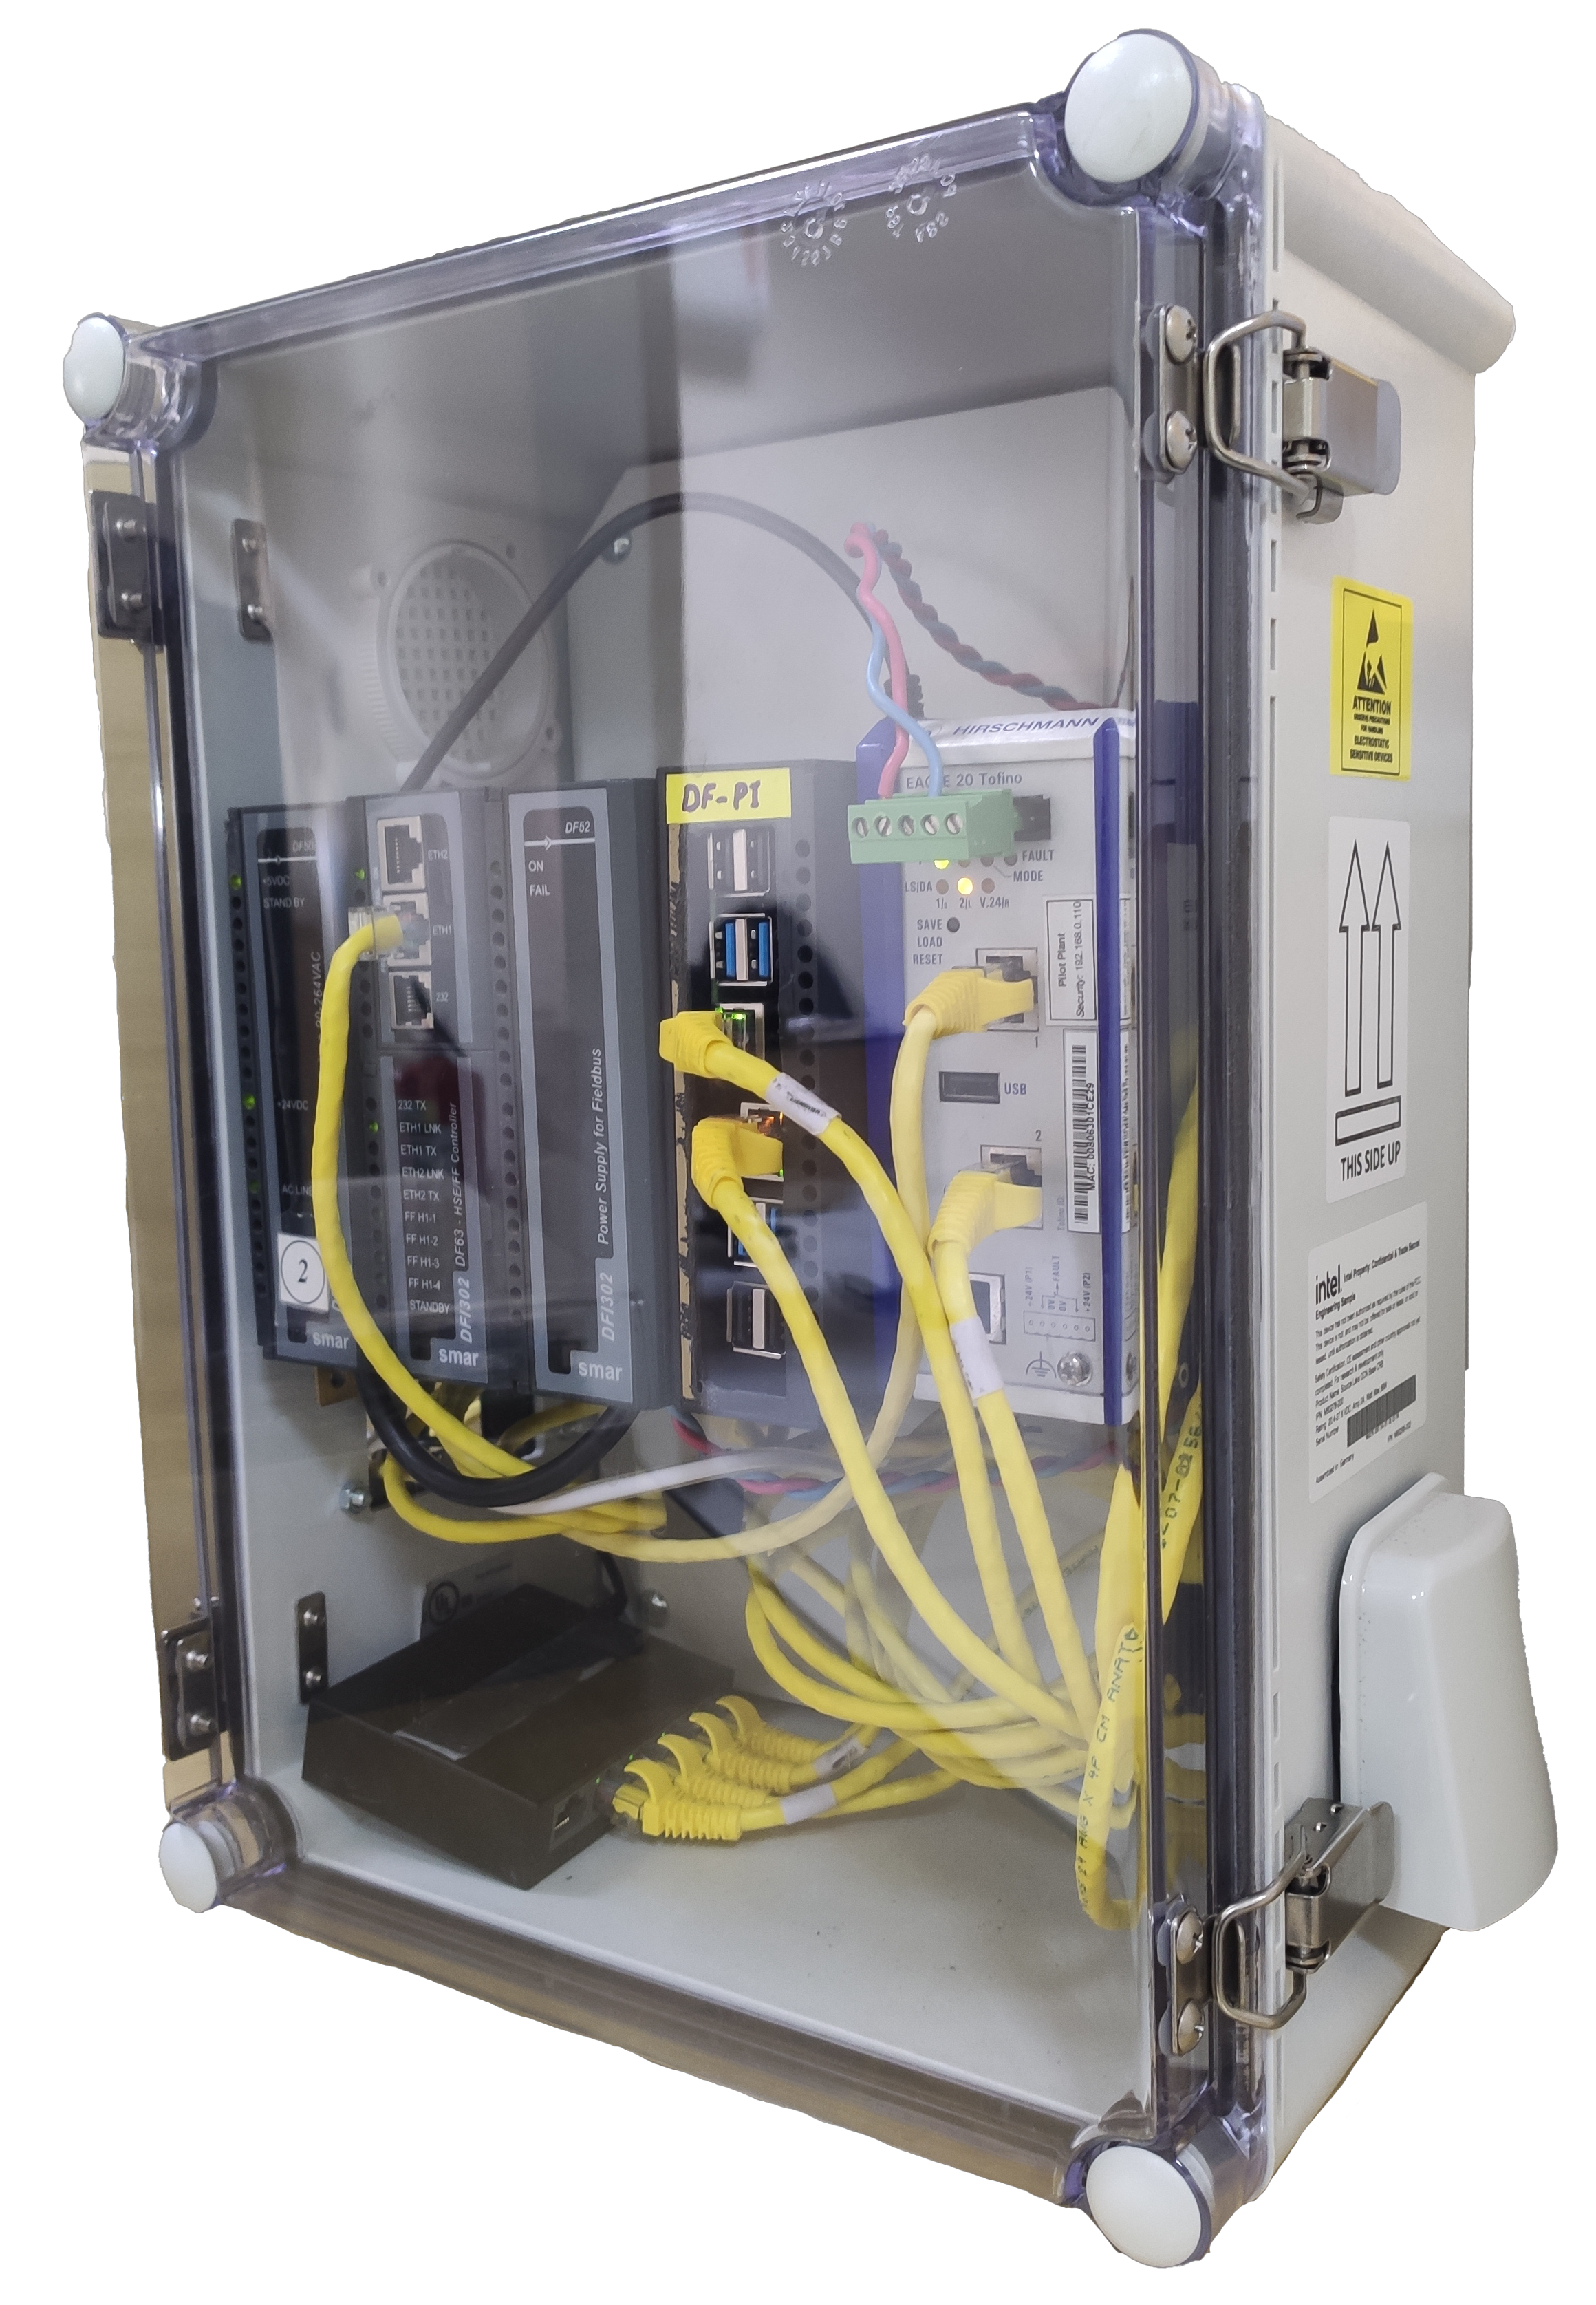
\includegraphics[width=0.5\textwidth]{USPSC-img/cyberkit2.png}
        \end{center}
        \legend{Fonte: elaborada pelo autor.}
    \end{figure}

\section{Ataques Cibernéticos em Redes Industriais OPC UA} \label{sec:attacks}

    Nesta seção, uma análise detalhada dos cenários de ataque implementados minuciosamente no âmbito do presente projeto é apresentada. A exposição abrangente engloba uma descrição passo a passo das metodologias empregadas para orquestrar três formas distintas de ciberataques: \textit{sniffing} de pacotes (do inglês \textit{Packet Sniffing}), ataques do tipo MITM e de negação de serviço. Ao elucidar as complexidades destes vetores de ataque, objetiva-se proporcionar uma compreensão profunda do cenário em evolução das ameaças à cibersegurança em redes OPC UA.

    \subsection{\textit{Packet Sniffing}}

    Uma vez que a rede OPC UA esteja instalada e funcionando em seus respectivos dispositivos, o Elemento Invasor inicia o \textit{software} Ettercap e o utiliza como um \textit{sniffer} unificado para obter informações detalhadas sobre os alvos disponíveis na rede. O modo unificado do Ettercap permite a execução do ataque por uma única interface de rede. É importante observar que o Elemento Invasor deve estar configurado na mesma rede de comunicação OPC UA e conectado a uma porta do \textit{switch} gerenciável, que por sua vez, replica o tráfego de dados das outras portas (do componente cliente e servidor OPC UA), conforme ilustrado na \autoref{fig:sniffing}. 

    \begin{figure}[htbp]
        \caption{\label{fig:sniffing}Esquemático do ataque \textit{Packet Sniffing}}
        \begin{center}
            \includegraphics[width=0.9\textwidth]{USPSC-img/sniffing-low.png}
        \end{center}
        \legend{Fonte: elaborada pelo autor.}
    \end{figure}
    
    Com o \textit{sniffing} de rede iniciado pelo Ettercap, utiliza-se o Wireshark para analisar mais detalhes sobre os endereços obtidos. A \autoref{fig:sniffWire} apresenta a série de pacotes que o \textit{software} disponibiliza quando a operação de \textit{sniffing} do tráfego de rede é bem-sucedida. Maiores detalhes da análise aplicada nos dados obtidos nesse processo são apresentados no \autoref{cap:resultados}.

    \begin{figure}[htbp]
        \caption{\label{fig:sniffWire}Resultados de captura do Wireshark durante o \textit{sniffing} de pacotes}
        \begin{center}
            \includegraphics[width=1\textwidth]{USPSC-img/sniffWire.png}
        \end{center}
        \legend{Fonte: elaborada pelo autor.}
    \end{figure}
    
    Os detalhes dos pacotes capturados pelo Wireshark são analisados e descritos detalhadamente no \autoref{cap:resultados}.
    
    \subsection{\textit{Man in The Middle (MITM)}}

    Ao efetuar esse ataque, o Elemento Invasor pode interceptar as informações do \textbf{SecureChannel} entre o cliente e servidor OPC UA, como mostra a \autoref{fig:mitm}.

    \begin{figure}[htbp]
        \caption{\label{fig:mitm}Esquemático do ataque MITM}
        \begin{center}
            \includegraphics[width=0.9\textwidth]{USPSC-img/mitm-low.png}
        \end{center}
        \legend{Fonte: elaborada pelo autor.}
    \end{figure}
    
    A primeira ferramenta de software utilizada nesse processo é a Ettercap, utilizada para realizar uma varredura da rede. Ao iniciar a busca direta por \textit{hosts} ativos, todos os endereços da máscara de rede são verificados a fim de identificar quais deles estão em funcionamento. Como exemplo, caso a máscara de rede configurada seja 255.255.255.0 (24), um total de 256 endereços são varridos.
    
    Após o término dessa operação de varredura, o Elemento Invasor pode selecionar o(s) alvo(s) nos quais receberam o ataque MITM e então, prosseguir com o `envenenamento' da rede por ARP (do inglês \textit{ARP Spoofing}), um dos tipos mais comuns de efetuar esse ataque. O ARP (do ingês \textit{Address Resolution Protocol}) é um dos protocolos de comunicação mais importantes da camada de rede do modelo OSI, utilizado para determinar o endereço MAC (do inglês \textit{Media Access Control}) de um dispositivo com base no seu endereço IP. Com o \textit{ARP Spoofing}, o invasor é capaz de anunciar à rede que o seu endereço MAC é o correto para os endereços IP pertencentes ao roteador e à estação de trabalho. Assim, estes dois dispositivos atualizam as suas entradas de cache ARP, e, a partir desse ponto, comunicam-se com o invasor, em vez de diretamente entre si.

    Enquanto o \textit{ARP Spoofing} é realizado pela ferramenta Ettercap, inicia-se a captura de pacotes pelo Wireshark. Para facilitar a visualização e a análise realizada neste estudo, o Wireshark é configurado para o protocolo OPC UA, permitindo um exame detalhado da comunicação entre os dispositivos na rede.
    
    \subsection{\textit{Denial of Service (DoS)}}

    Esse tipo de ataque possibilita a inserção de clientes não confiáveis na rede OPC UA pelo Elemento Invasor, assim como uma inundação da rede e do servidor ao enviar mensagens específicas continuamente. A \autoref{fig:dos} apresenta um esquemático básico de um funcionamento de DoS, nas quais as solicitações advindas de um cliente OPC UA não confiável são interpretadas pelo servidor, mas não são aceitas pelo remetente devido à sua falsificação de endereço.

     \begin{figure}[htbp]
        \caption{\label{fig:dos}Esquemático do ataque DoS}
        \begin{center}
            \includegraphics[width=0.9\textwidth]{USPSC-img/dos-low.png}
        \end{center}
        \legend{Fonte: elaborada pelo autor.}
    \end{figure}
    
    Existem diversos cenários possíveis para a efetuação do ataque de negação de serviço. Além do impacto da inundação na rede, ressaltam-se os efeitos no processamento do componente ao sofrer ataques intensivos, nos quais os servidores precisam avaliar as certificações para responderem solicitações. Segundo \citeonline{neu2019}, os principais cenários são:

    \begin{enumerate}
        \item \underline{SYN \textit{Flooding}}: o cliente sobrecarrega o servidor enviando mensagens SYN de forma contínua, e o servidor responde com ACK a cada uma dessas mensagens. Embora essa ação possa inundar a rede com tráfego sobrecarregado com estas mensagens, seu impacto no consumo de recursos do servidor é limitado;
        \item \underline{ACK ou ERR \textit{Flooding}}: nesse cenário, o cliente inunda o servidor com mensagens ACK e/ou ERR, às quais o servidor responde com mensagens ERR. Da mesma forma do anterior, pode haver sobrecarga na rede, mas possui impacto moderado nos recursos do servidor;
        \item \underline{Inundação com Mensagens Incorretas}: são enviadas continuamente mensagens incorretas pelo Elemento Invasor, forçando respostas ERR pelo servidor. Também cria-se sobrecarga na rede, mas apresenta impacto relativamente baixo no processamento do servidor;
        \item \underline{CLO \textit{Flooding}}: enviam-se, repetidamente, mensagens de solicitação de fechamento de canal (CLO) ao servidor, que responde com mensagens ERR, sobrecarregando a rede com o tráfego destas mensagens.
        \item \underline{Inundação com \textbf{FindServers} ou \textbf{GetEndpoints}}: O cliente estabelece um canal no modo de segurança \textbf{None} e, em seguida, envia continuamente mensagens \textbf{FindServers()} ou \textbf{GetEndpoints()} para o servidor, que, por sua vez, responde com as mesmas mensagens por meio do OPC UA MSG. Apesar de apresentar impacto na rede, não altera os recursos do servidor;
        \item \underline{Inundação com Solicitações SYN e OPN}: um cliente não confiável realiza um ataque de negação de serviço enviando continuamente solicitações SYN e OPN ao servidor. O servidor responde com mensagens ACK e ERR. Nesse ataque, o servidor consome recursos substanciais durante a validação do certificado, na solicitação e no processo de criptografia da mensagem. Esse ataque pode ser ainda mais eficaz quando a Autoridade de Certificação está localizada em um sistema diferente, aumentando consideravelmente o tempo de validação do certificado, e, consequentemente, o processamento do componente onde se encontra o servidor.
    \end{enumerate}

    Duas ferramentas são utilizadas para efetuar a inundação da rede e, assim, alcançar o DoS: OPC UA Exploit Framework e Hping3, além de aplicar o Nmap para efetuar uma varredura da rede a fim de encontrar portas abertas e endereços IP disponíveis. 

    Uma vez que o Elemento Invasor obteve acesso a algum dos componentes da rede do alvo, o Nmap é utilizado para mapeamento da rede em questão. O comando abaixo executa um \textit{scan} SYN em um range de IPs, relativamente não-obstrusivo e camuflado, uma vez que ele nunca completa uma conexão TCP. Também chamado de escaneamento de portas entreabertas (\textit{half-open scanning}), um pacote SYN é enviado como se fosse abrir uma conexão real, cuja espera-se uma resposta. Um SYN/ACK indica que a porta está ouvindo (aberta), enquanto um RST (\textit{reset}) é indicativo de uma não-ouvinte. Se nenhuma resposta é recebida após diversas retransmissões, a porta é marcada como filtrada. A porta também é marcada como filtrada se um erro ICMP de inalcançável é recebido.

    \begin{minted}[
        breaklines,
        %linenos,
        mathescape,
        encoding=utf8,
        framesep=2mm,
        baselinestretch=1.2,
        bgcolor=codeback,
        fontsize=\footnotesize
    ]{console}
Nmap -sS 192.168.164.*
    \end{minted}

    A correta execução desse mapeamento resulta em uma lista de IPs disponíveis e portas abertas, que servirão de entrada para os próximos passos. O Hping3 é utilizado para realizar o SYN \textit{Flooding} na rede. Para isso, o \textit{script} de configuração abaixo deve ser implementado pelo Elemento Invasor, customizando-o de acordo com cada cenário.

    \begin{minted}[
        breaklines,
        %linenos,
        mathescape,
        encoding=utf8,
        framesep=2mm,
        baselinestretch=1.2,
        bgcolor=codeback,
        fontsize=\footnotesize
    ]{bash}
# CONFIGURAÇÃO
set TARGET "192.168.164.101"  # O alvo do ataque
set FAKEIP "192.168.164.201"  # Endereço falso
set BROADCAST "192.168.164.254"  # Endereço de broadcast da rede

set PORTS {{4840}{4192}}  # Utilizar as portas abertas encontradas no Nmap
set PORTUDP 123  # Utilizar uma porta UDP ativa

set commandRunTime 180

# EXECUÇÃO
foreach port $PORTS {
    lappend commands "hping3 -S -a $FAKEIP -p $port --flood -V $TARGET"
}
    \end{minted}

    Com isso, o Hping3 está preparado para iniciar o ataque direcionado ao endereço e portas especificados, com uma frequência predefinida (neste caso, 180 segundos). A interpretação dos parâmetros utilizados na execução é a seguinte: o argumento \textbf{-S} define o tipo de ataque, \textbf{-p} identifica a porta de destino, \textbf{-V} indica o endereço IP do alvo, enquanto \textbf{-a} determina o endereço IP falsificado utilizado no ataque, uma estratégia que pode contornar \textit{firewalls} de forma eficaz.

    Por fim, alguns ataques mais robustos são efetuados com o auxílio da ferramenta OPC UA Exploit Framework. Os ataques de negação de serviço disponibilizados pelo \textit{framework} e escolhidos para execução no ambiente de simulação industrial proposto, são apresentados abaixo, seguidos de suas respectivas categorias, conforme os cenários supracitados e apresentados por \citeonline{neu2019}, e suas descrições:

    \begin{itemize}
        \item[N/A] \underline{Loop infinito na cadeia de certificados}: refere-se a uma situação em que alguns servidores implementam a verificação da cadeia de certificados por conta própria, sem proteção contra um loop de cadeia infinita. Isso pode ocorrer quando um certificado A, por exemplo, é assinado por outro certificado B, que por sua vez é assinado pelo A. Cria-se uma dependência circular entre os certificados A e B, resultando em um loop infinito durante o processo de verificação da cadeia de certificados;
        \item[(3)] \underline{Inundação por \textit{Chunk}}: envolve o envio de uma quantidade abundante de fragmentos de dados ao servidor sem o envio do fragmento final correspondente. O OPC UA permite a divisão dos dados em fragmentos, comumente chamados como \textit{MessageChunks} ou \textit{Chunks}, que são enviados à medida que são codificados, a fim de facilitar a transmissão e o processamento. Caso ocorra um erro na criação de um destes fragmentos, um \textit{Chunk} final deve ser enviado ao destinatário para notificar o erro, que por sua vez, é marcado com um sinalizador `A' (abortar) para indicar o erro. O receptor deve verificar a segurança do \textit{MessageChunk} abortado antes de processá-lo e, caso esteja tudo certo, ignorar a mensagem, mas sem encerrar o \textbf{SecureChannel};
        \item[(6)] \underline{Abertura de múltiplos canais seguros}: tentativa de inundação do servidor com uma quantidade abundante de solicitações \textbf{OpenSecureChannels};
        % \item[(3)] \underline{Mensagem aninhada complexa}: aplicação de uma variante especialmente manipulada e complexa, projetada para explorar vulnerabilidades em um servidor OPC UA. Quando esta variante é processada pelo servidor, ela pode causar um estouro na pilha de chamadas (\textit{call stack overflow}), levando a uma falha no servidor;
        \item[(5)] \underline{Tradução do caminho de navegação}: são enviadas ao servidor requisições de traduções de \textit{browse path} complexas que exploram a falta de limites adequados na resolução destes caminhos, podendo causar também um \textit{call stack overflow};
        % \item[Não aplicável] \underline{Falha de espera no \textit{Thread Pool}}: caracteriza uma paralisação (\textit{deadlock}) no sistema de \textit{Thread Pool} -- mecanismo de gerenciamento de \textit{threads} utilizado para processar solicitações de clientes e tarefas no servidor OPC UA -- devido à inanição simultânea de tarefas concorrentes. Em termos mais simples, quando vários processos ou \textit{threads} estão competindo por recursos do \textit{Thread Pools} de um servidor e, devido a problemas de sincronização ou gerenciamento inadequado de \textit{threads}, ficam em um estado de espera prolongado, impedindo efetivamente o servidor de processar solicitações legítimas;
        % \item[(6)] \underline{Persistência ilimitada de subscrições}: inúmeras solicitações de monitoramento ao servidor são enviados por um invasor, todas configuradas para não excluir os itens após o monitoramento. Esta persistência resulta em uma alocação descontrolada de recursos de memória pelo servidor, levando eventualmente a uma negação de serviço devido ao esgotamento de recursos.
        % \item[(3)] \underline{Chamada da função \textit{Dereference} nula}: envolve a chamada de vários métodos OPC UA e encerramento da sessão antes da conclusão destes. Isso resulta em uma situação em que a aplicação servidora é forçada a referenciar um objeto nulo ou um ponteiro invalido, levando a um erro de execução;
        % \item[(3)] \underline{Alteração de corrida e navegação no espaçamento de endereço}: o Elemento Invasor realiza a adição de \textit{Nodes} no \textit{Address Space} no servidor e, simultaneamente, remove-os em um ciclo contínuo, enquanto percorre todo o espaçamento de endereço. Esta manobra cria uma situação de competição na qual o servidor está sendo constantemente modificado e examinado ao mesmo tempo, podendo, assim, esgotar os recursos de processamento e resultar em problemas de consistência no \textit{Address Space};
        % \item[(6)] \underline{Atualização de condição ilimitada}: refere-se ao envio repetido e quantidade abundante de chamadas do método \textbf{ConditionRefresh}, o que leva a alocações de memória não controladas e, eventualmente, pode resultar em uma falha no sistema. O método ConditionRefresh é usado para atualizar as condições e estados das variáveis monitoradas em um servidor OPC UA.
    \end{itemize}

    Sabendo disso, os ataques acima podem ser efetuados através da seguinte linha de comando base, substituindo SERVER\_TYPE pelo tipo de servidor utilizado (\textit{e.g.}, softing, unified, prosys, kepware, triangle, dotnetstd, open62541, ignition, rust, node-opcua, opcua-python, milo e s2opc), IP\_ADDR pelo endereço de IP do alvo, PORT pela porta aberta para a comunicação UA, ENDPOINT\_ADDRESS pelo endpoint do servidor, FUNC\_TYPE pelo tipo de ataque escolhido (verificar na documentação oficial do framework \cite{claroty2023}, quais os nomes das funções disponíveis) e DIR, necessário para algumas funções:

    \begin{minted}[
        breaklines,
        %linenos,
        mathescape,
        encoding=utf8,
        framesep=2mm,
        baselinestretch=1.2,
        bgcolor=codeback,
        fontsize=\footnotesize
    ]{console}
python main.py [SERVER_TYPE] [IP_ADDR] [PORT] [ENDPOINT_ADDRESS] [FUNC_TYPE] [DIR*]
    \end{minted}

\section{Metodologia}

    O fluxograma apresentado na \autoref{fig:flux} explicita a sequência e estrutura de atividades, os passos que compõem a metodologia, posteriormente explicados nas subseções.
    
    \begin{figure}[htbp]
        \caption{\label{fig:flux}Fluxograma da metodologia proposta}
        \begin{center}
            \includegraphics[width=0.7\textwidth]{USPSC-img/fluxograma-low.png}
        \end{center}
        \legend{Fonte: elaborada pelo autor.}
    \end{figure}

    Para a realização adequada do experimento proposto neste estudo, a infraestrutura de rede do protocolo OPC UA foi configurada conforme os seguintes parâmetros: um dos Raspberry Pi e a DF63 NG atuaram como servidores, enquanto a outro Raspberry Pi desempenhou o papel de cliente. Além disso, um elemento de rede chamado `Sniffer' (conforme ilustrado na \autoref{fig:banc}) foi inserido na configuração para monitorar e registrar a comunicação da rede. Com o propósito de fornecer uma visão clara dos componentes envolvidos e facilitar a análise dos dados coletados durante o experimento, os endereços IP e MAC de cada elemento do sistema estão resumidos na \autoref{tab:ender}. Importante mencionar que os servidores OPC UA foram configurados para utilizar a porta padrão 4840, e os endpoints correspondentes também são apresentados ao lado de seus respectivos elementos. Essa estrutura de configuração foi essencial para a condução eficaz do experimento e a subsequente análise dos resultados.

    \begin{table}[htbp]
        \centering
        \caption{Endereços IP e MAC dos equipamentos da rede OPC UA}%
	\label{tab:ender}
        \begin{tabular}{cccc}
            \toprule
            \thead{Equipamento} & \thead{IP} & \thead{MAC} & \thead{OPC UA Endpoint} \\
            \toprule
            DF63 NG  & 192.168.164.100 &  & \\
            \midrule
            RaspPi 1 & 192.168.164.101 & E4:5F:01:2E:1A:B6 & \\
            \midrule
            RaspPi 2 & 192.168.164.102 & E4:5F:01:2E:1B:C1 & \\
            \midrule
            Sniffer  & 192.168.164.201 & C8:3A:35:49:FD:58 & \\
            \midrule
            Invasor  & 192.168.164.200 &  & \\
            \bottomrule
        \end{tabular}
        \fonte{elaborada pelo autor.}%
    \end{table}

    \subsection{Aquisição de Dados}

    A fase de aquisição de dados fundamenta-se na captura do tráfego de pacotes transmitidos pela rede OPC UA durante a comunicação entre a aplicação servidora e o cliente da rede, durante a execução dos ataques. Esse processo se baseia na utilização do software Wireshark, no qual permite a coleta de informações cruciais sobre a comunicação, incluindo detalhes como o tipo de protocolo empregado e a origem e o destino dos dados. As informações capturadas são armazenadas em ordem cronológica com a capacidade de serem salvas em arquivos no formato `.pcapng'. O software Wireshark está configurado para atualizar a captura a cada segundo.

    Os alvos dos ataques são os servidores OPC UA, e em cada cenário, o elemento \textit{Sniffer} é configurado para realizar a captura do tráfego gerado por estes ataques. Para organizar os pacotes capturados, foi adotada a seguinte nomenclatura de arquivos: `[Modo de Segurança]-[Tipo do Ataque]-[Número da Captura].pcapng'. Aqui, o modo de segurança pode assumir os valores 0 (None), 1 (Sign) e 2 (Sign\&Encrypt). Os tipos de ataques correspondem àqueles detalhados na \autoref{sec:attacks} (`sniffing', `mitm' e `dos-[função]'), e o número da captura é representado por um dígito de 0 a 9. Por exemplo, para salvar a terceira captura obtida durante uma negação de serviço pelo ataque \textit{Chunk Flooding}, com a rede configurada no modo de segurança \textbf{Sign}, o arquivo seria nomeado como: `1-dos-chunkflood-3.pcapng'.

    Além disso, é importante salientar que durante o processo de coleta de dados com o Wireshark, simultaneamente, obtêm-se informações sobre a carga de processamento da CPU nos hospedeiros do servidor OPC UA. Essa abordagem complementa significativamente a análise dos efeitos do ataque sobre o desempenho do sistema. Para viabilizar esse monitoramento, desenvolveu-se um \textit{script} que deve ser ativado pelo elemento \textit{Sniffer} no início da captura de dados. Essa avaliação detalhada contribui para uma compreensão mais completa e precisa dos efeitos das ameaças cibernéticas na infraestrutura OPC UA em análise.

    \begin{minted}[
        breaklines,
        %linenos,
        mathescape,
        encoding=utf8,
        framesep=2mm,
        baselinestretch=1.2,
        bgcolor=codeback,
        fontsize=\footnotesize
    ]{bash}
#!/bin/bash

output_file="0-dos-chunkflood-3.csv"

if [ ! -e "$output_file" ]; then
    echo "Timestamp (s),RAM (%),CPU (%),Disco (%)" > "$output_file"
fi

# Obter diagnóstico por 1 minuto
duration=60
start_time=$(date +%s)

while true; do
    timestamp=$(date +"%Y-%m-%d %H:%M:%S")
    
    # Porcentagem de uso da RAM
    ram_usage=$(free | awk '/Mem/ {print $3/$2 * 100.0}')
    
    # Porcentagem de uso do CPU
    cpu_usage=$(top -bn1 | grep "Cpu(s)" | awk '{print $2}' | awk -F. '{print $1}')
    
    # Porcentagem de uso do disco para o sistema de arquivos do root ("/")
    disk_usage=$(df -h / | awk 'NR==2 {print $5}' | sed 's/%//')
    
    echo "$timestamp,$ram_usage,$cpu_usage,$disk_usage" >> "$output_file"

    current_time=$(date +%s)

    if [ $((current_time - start_time)) -ge $duration ]; then
        break
    fi
    
    # Escala de 1 segundo
    sleep 1
done

echo "Diagnóstico finalizado. Dados salvos no arquivo $output_file"
    \end{minted}
    
    % \subsection{Interpretação dos Dados}

    % Uma vez que os ataques são coletados e salvos nos arquivos de capturas, 

    % \subsection{Análise de Ataques e Vulnerabilidades}

    % \subsection{Contramedidas de Segurança}